\documentclass[10pt]{article}
\usepackage[polish]{babel}
\usepackage[utf8]{inputenc}
\usepackage[T1]{fontenc}
\usepackage{amsmath}
\usepackage{amsfonts}
\usepackage{amssymb}
\usepackage[version=4]{mhchem}
\usepackage{stmaryrd}
\usepackage{graphicx}
\usepackage[export]{adjustbox}
\graphicspath{ {./images/} }

\title{KLASY PIERWSZE I DRUGIE }

\author{}
\date{}


\begin{document}
\maketitle
\begin{enumerate}
  \item Udowodnij, że dla każdej liczby pierwszej \(p\) większej od 3 liczba \(p^{2}-1\) jest podzielna przez 24.
  \item Wyznacz liczbę par \((x, y)\) liczb całkowitych spełniających równanie
\end{enumerate}

\[
x^{4}=y^{4}+1223334444
\]

\begin{enumerate}
  \setcounter{enumi}{2}
  \item Czworokąt wypukły podzielono na cztery części łącząc środki jego boków jak na rysunku. Wykaż, że suma pól części zacienionych jest równa sumie pól części niezacienionych.\\
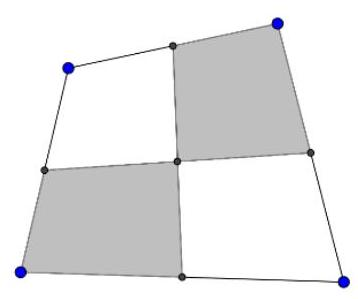
\includegraphics[max width=\textwidth, center]{2024_11_21_a2b9e49dabde1310792eg-1(1)}
\end{enumerate}

\section*{KLASY TRZECIE I CZWARTE}
\begin{enumerate}
  \item Udowodnij, że jeżeli przez punkt H przechodzą trzy okręgi o jednakowych promieniach, a punkty \(\mathrm{A}, \mathrm{B}, \mathrm{C}\) są różnymi od H punktami przecięć tych okręgów, to H jest ortocentrum trójkąta ABC .
  \item Na rysunku punkty A' i B' są spodkami wysokości, a punkt M jest środkiem boku AB. Udowodnij, że punkt M jest środkiem łuku \(A^{\prime} B^{\prime}\) okręgu dziewięciu punktów trójkąta ABC.\\
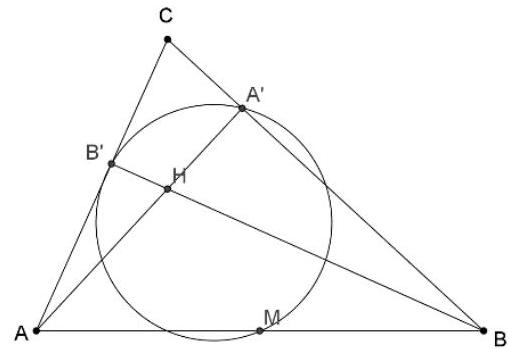
\includegraphics[max width=\textwidth, center]{2024_11_21_a2b9e49dabde1310792eg-1(2)}
  \item Odcinek \(A B\) ślizga się po ramionach kąta prostego w ten sposób, że punkt \(A\) należy do jednego ramienia, a punkt \(B\) do drugiego. Jaki kształt będzie miała droga, którą przebędzie środek odcinka \(A B\). Odpowiedź uzasadnij.\\
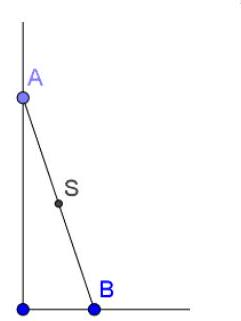
\includegraphics[max width=\textwidth, center]{2024_11_21_a2b9e49dabde1310792eg-1}
\end{enumerate}

\end{document}